\chapter{Application Examples}

\begin{figure}[h]
\centering
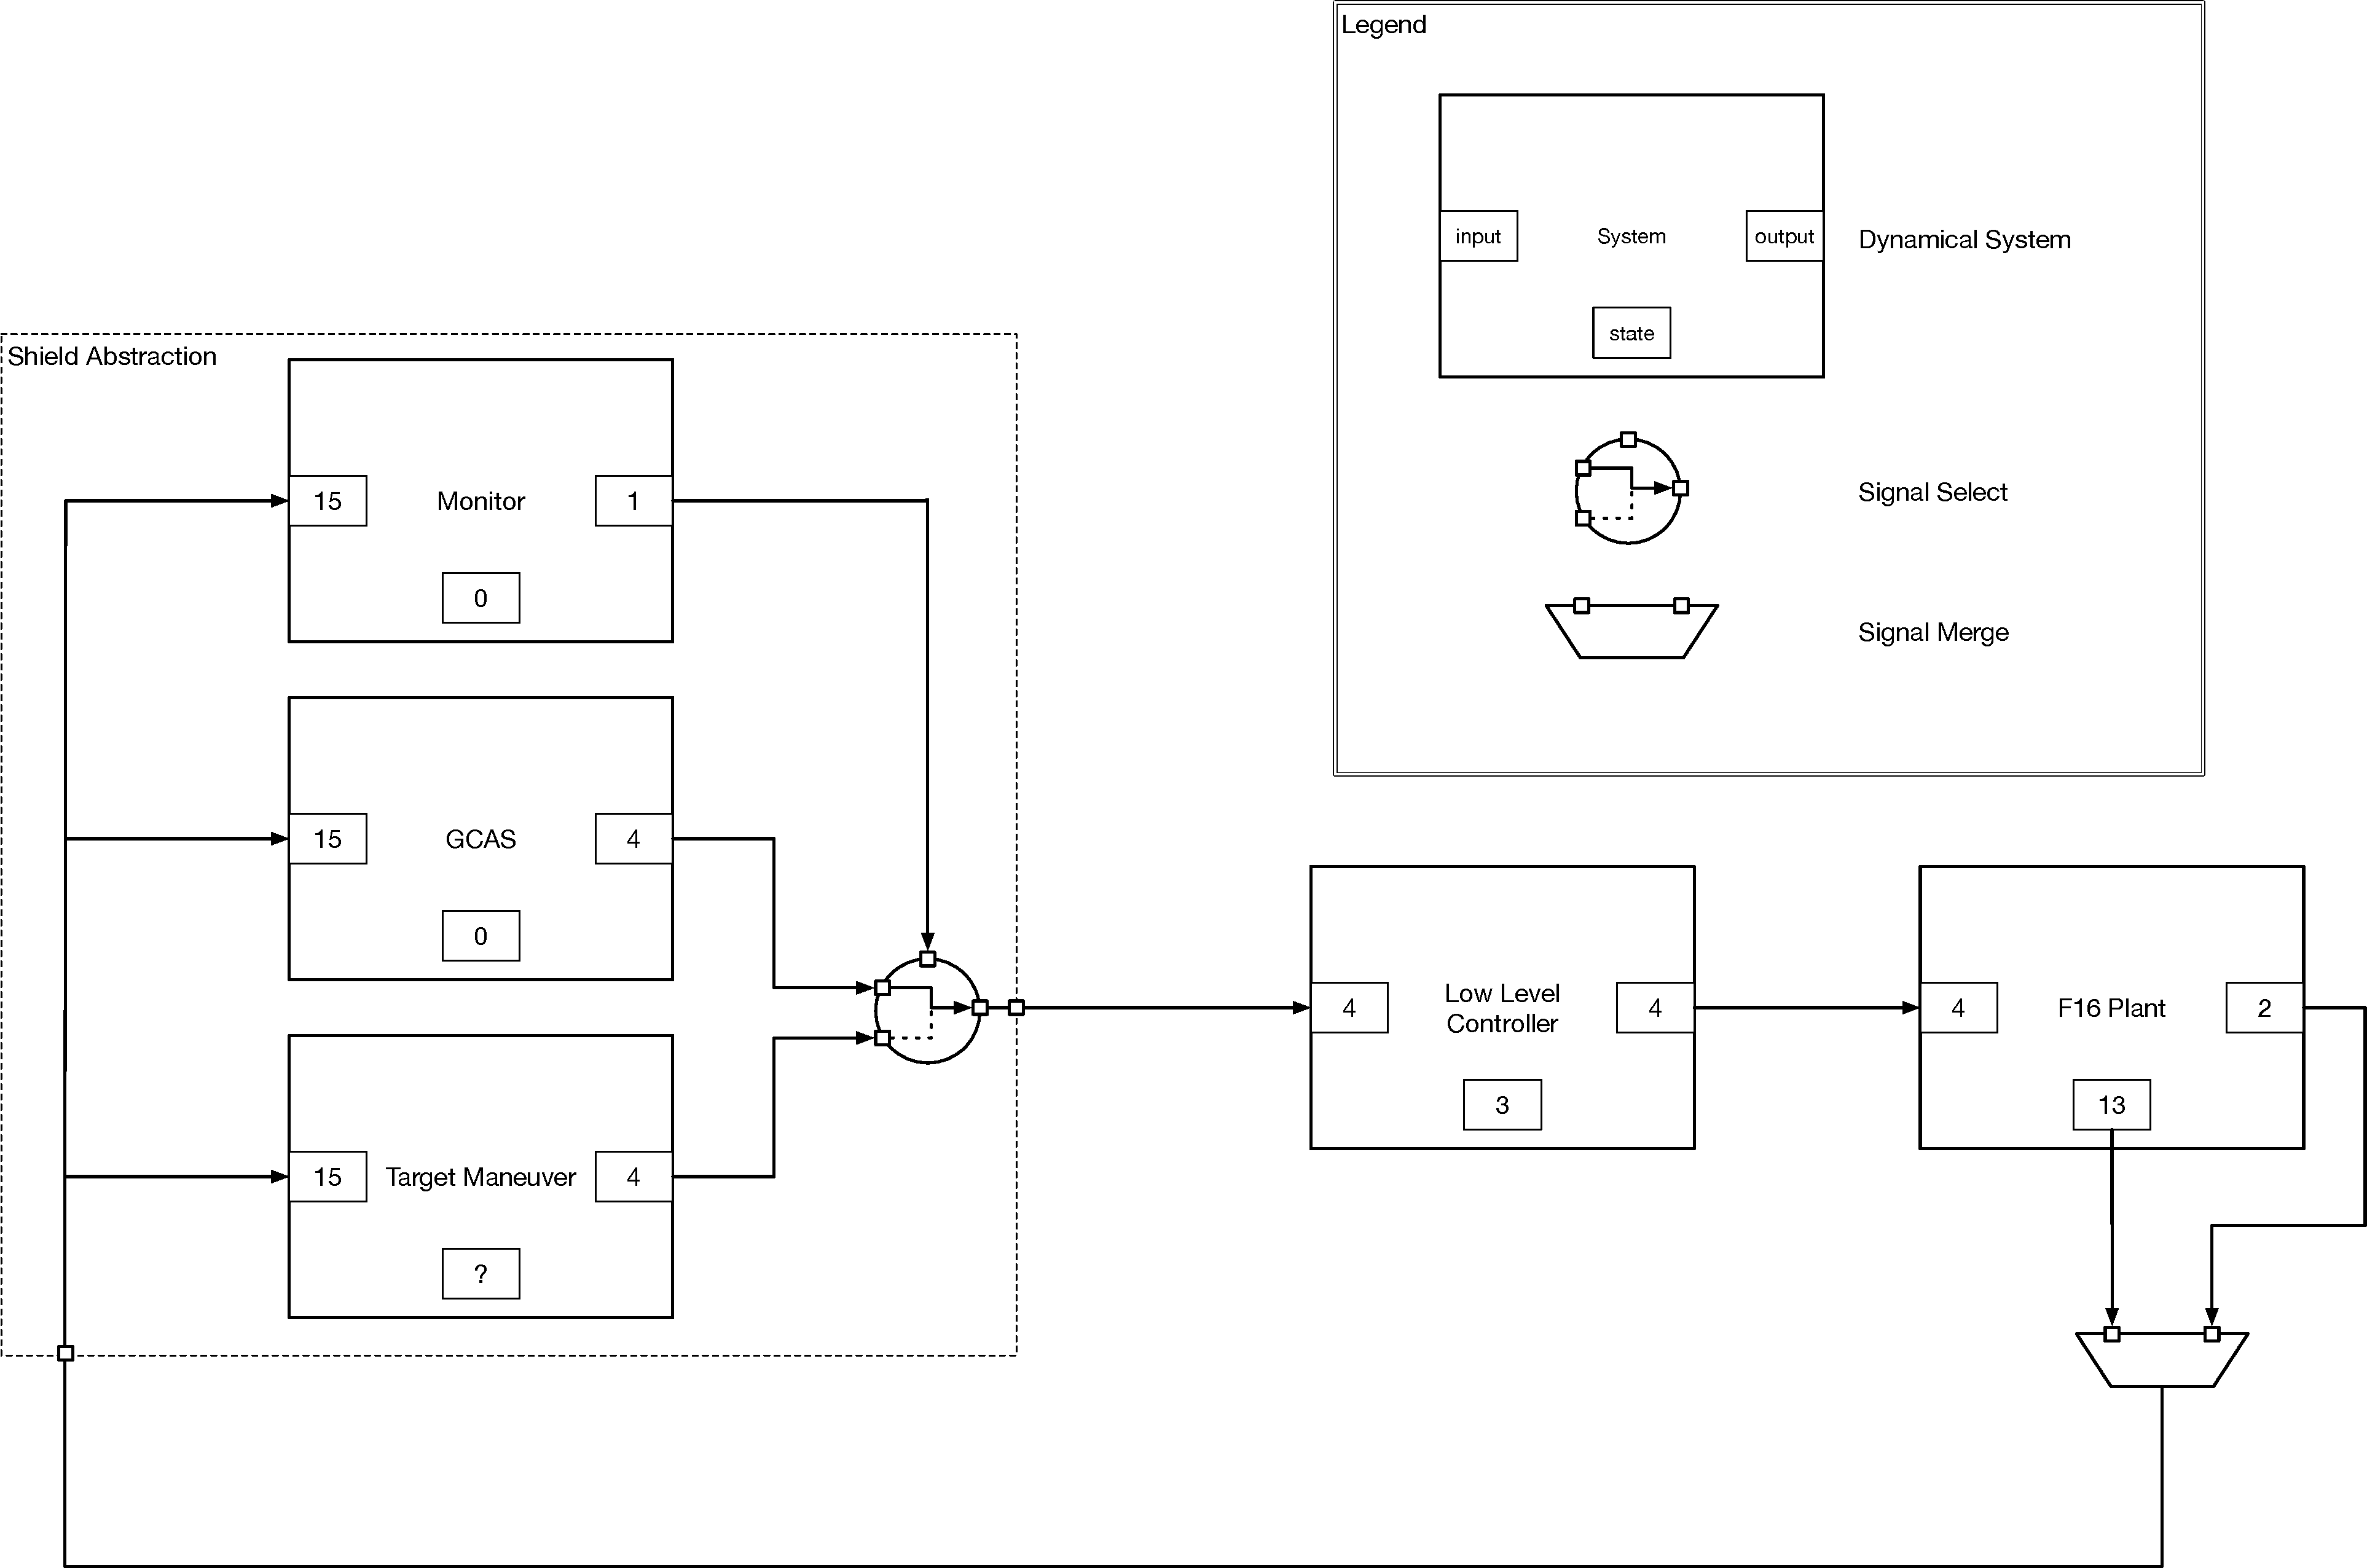
\includegraphics[width=\linewidth]{./img/f16demoblock.pdf}
\caption{Example Shield Configuration for a Controlled F-16 Model Used in Demo}
\label{fig:f16demoblock}
\end{figure}

\section{F-16 Model}

The flagship use of \acrshort{csaf} is a benchmark F16 fighting falcon model. It serves as an advanced model to develop 
offline and online control assurance schemes. The hope is to provide a benchmark to motivate better 
verification and analysis methods, working beyond models based on Dubins car dynamics, towards the sorts of 
models used in aerospace engineering. Roughly speaking, the dynamics are nonlinear, have about 10-20 
dimensions (continuous state variables), and hybrid in the sense of discontinuous \acrshort{ode}s, but not with jumps in 
the state. \\

A demonstration was created to show how the controllers can be swapped and recompose to alter flight 
trajectories. Figure \ref{fig:f16demoblock} shows an example control system for a \acrlong{gcas} shield. The 
model and \acrshort{gcas} problem is implemented \href{https://github.com/stanleybak/AeroBenchVVPython}
{here} and a theoretical perspective is offered in a paper \cite{heidlauf2018verification}. Target maneuvers are shielded by ground collision avoidance and the inner loop is using the classical controller with this configuration. For the demo, the outer loop is stateless, while the inner loop has three states for tracking. All of the system blocks are directly transferable to \acrshort{csaf} components.

\subsection{Example Messages}

To show translation to components, the associated message with the pub/sub elements can be formulated. 

\begin{figure}[h]
\centering
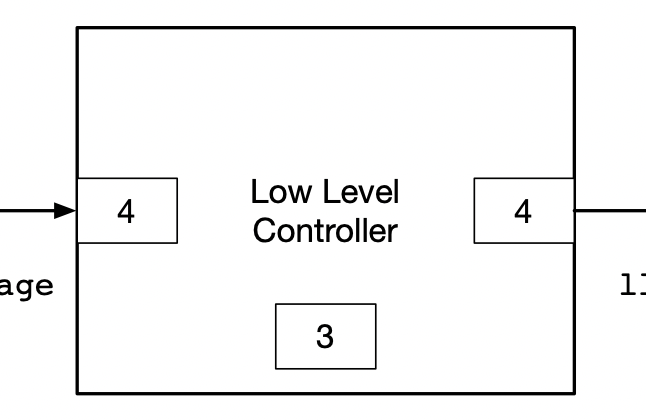
\includegraphics[width=0.5\linewidth]{./img/llc}
\caption{F-16 Controller}
\label{fig:f16plant}
\end{figure}

\subsubsection*{Temporal Message}

\textbf{state}
\begin{lstlisting}	
uint32 version_major
uint32 version_minor

string topic

float64 time

float64 int1
float64 int2
float64 int3
\end{lstlisting}

\textbf{output}
\begin{lstlisting}
uint32 version_major
uint32 version_minor

string topic

float64 time

float64 delta_e
float64 delta_a
float64 delta_r
float64 throttle
\end{lstlisting}

\subsubsection*{Component Configuration}

\begin{lstlisting}	
system_name = "F16 Low Level Controller"
system_representation = "black box"
system_solver = "Euler"

sampling_frequency = 100

is_discrete = false
is_hybrid = false

[parameters]
  K_lqr = [ [-156.9,  -31.0,  -38.7, 0.0, 0.0, 0.0, 0.0, 0.0],
            [ 0.0, 0.0, 0.0, 30.5, -5.71, -9.31, -34.0, -10.7],
            [0.0, 0.0, 0.0,-22.7,-14.2, 6.74, -53.7]]
  xequil = [502.0, 0.039, 0.0, 0.0, 0.039, 0.0, 0.0, 0.0, 0.0, 
  				0.0, 0.0, 1000.0, 9.06]
  uequil = [0.139, -0.750, 0.0, 0.0]
  throttle_max = 1
  throttle_min = 0
  elevator_max = 25
  elevator_min = -25
  aileron_max = 21.5
  aileron_min = -21.5
  rudder_max = 30.0
  rudder_min = -30.0

[inputs]
  msgs = [ "f16plant_state.msg", "f16plant_output.msg", 
  				"autopilot_output.msg" ]

[topics]

  [topics.outputs]
    msg = "f16llc_output.msg"

  [topics.states]
    msg = "f16llc_state.msg"
    initial = [ 0.0, 0.0, 0.0 ]
\end{lstlisting}
%
%
%\begin{figure}[h]
%\centering
%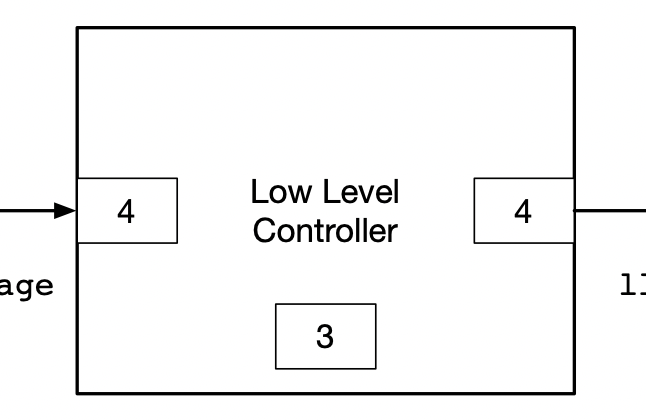
\includegraphics[width=0.5\linewidth]{./img/llc}
%\caption{F-16 Low Level Controller}
%\label{fig:f16plant}
%\end{figure}
%
%\begin{figure}[h]
%\centering
%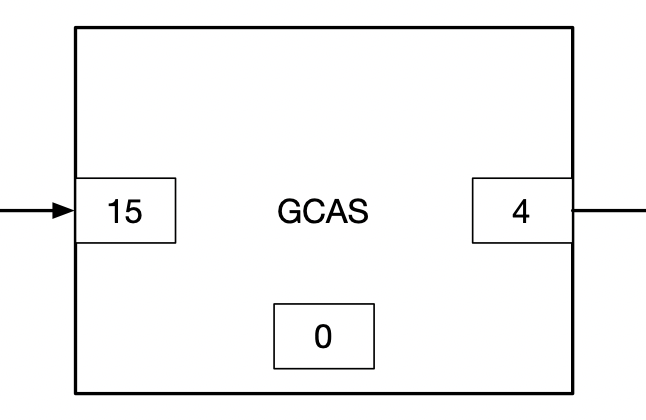
\includegraphics[width=0.5\linewidth]{./img/gcas}
%\caption{GCAS Maneuver Controller}
%\label{fig:f16plant}
%\end{figure}
%
%\begin{figure}[h]
%\centering
%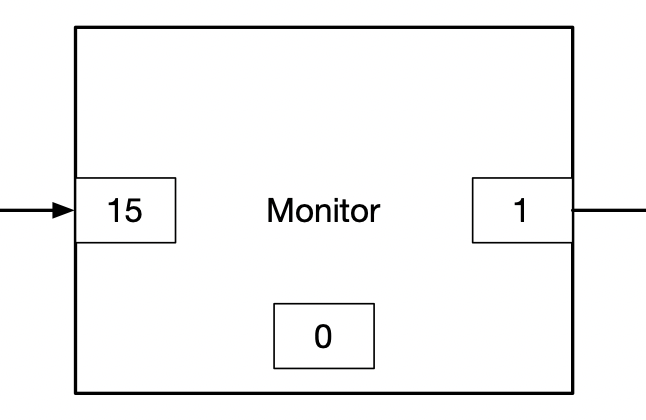
\includegraphics[width=0.5\linewidth]{./img/monitor}
%\caption{Outer Loop Monitor}
%\label{fig:f16plant}
%\end{figure}

